% Copyright 2019 the authors. All rights reserved.

% TODO:
% -

\documentclass[modern]{aastex62}

\usepackage{amsmath}

% typography
\setlength{\parindent}{1.\baselineskip}
\newcommand{\acronym}[1]{{\small{#1}}}
\newcommand{\package}[1]{\textsl{#1}}
\newcommand{\gaia}{\textsl{Gaia}}
\newcommand{\pans}{\textsl{Pan-STARRS}}
\newcommand{\DR}{\acronym{DR2}}
\newcommand{\msun}{\textrm{M}_\odot}
\newcommand{\kpc}{\textrm{kpc}}
\newcommand{\kms}{\ensuremath{\textrm{km}~\textrm{s}^{-1}}}
\newcommand{\bs}[1]{\boldsymbol{#1}}
\newcommand{\masyr}{\ensuremath{\textrm{mas}~\textrm{yr}^{-1}}}
\newcommand{\feh}{\ensuremath{[\textrm{Fe} / \textrm{H}]}}
\newcommand{\given}{\,|\,}


\newcommand{\sectionname}{Section}
\newcommand{\equationname}{Equation}
\renewcommand{\tablename}{Table}

\newcommand{\todo}[1]{{\color{red} TODO: #1}}

\newcommand{\changes}[1]{{\textbf{#1}}}
% \newcommand{\changes}[1]{{#1}}

% aastex parameters
% \received{not yet; THIS IS A DRAFT}
%\revised{not yet}
%\accepted{not yet}
% % Adds "Submitted to " the arguement.
% \submitjournal{ApJ}
\shorttitle{Stuff}
\shortauthors{People}

%@arxiver{}

\begin{document}\sloppy\sloppypar\raggedbottom\frenchspacing % trust me

\title{Flashy title}

% \author[0000-0003-0872-7098]{Adrian~M.~Price-Whelan}
% \affiliation{Department of Astrophysical Sciences,
%              Princeton University, Princeton, NJ 08544, USA}
% \email{adrn@astro.princeton.edu}
% \correspondingauthor{Adrian M. Price-Whelan}

% \author[0000-0002-7846-9787]{Ana Bonaca}
% \affiliation{Harvard--Smithsonian Center for Astrophysics, Cambridge, MA 02138, USA}

\begin{abstract}\noindent % trust me
    Words!
\end{abstract}

\keywords{Galaxy: halo --- dark matter ---
          Galaxy: kinematics and dynamics}

\section{Introduction}
\label{sec:intro}


\section{Data}
\label{sec:data}

\section{Simulations}
\label{sec:sim}
In order to explore the mechanism leading the the observed morphology of the stream (e.g. the length asymmetry between the leading and trailing arm, as well as the gap in the trailing arm, and the ``fan" in the leading arm), we run a suite of Pal 5 simulations. In particular, we investigate whether Pal 5's ``fan" in the leading arm can be explained from mild chaos  (\citealt{Pearson:2015}, \citealt{Price-Whelan:2016}), or whether Pal 5 is interacting with the Galactic bar (\citealt{Pearson:2017}, \citealt{Erkal:2017}, \citealt{Banik:2019}). In Section \ref{sec:potential}, we describe the potentials in which we simulate the evolution of Pal 5, and in Section \ref{sec:potential} we describe our suite of Pal 5 stream simulations. 

\subsection{Potential}
\label{sec:potential}
We simulate the evolution of Pal 5 in two classes of three-component Galactic potentials: 

\begin{itemize}
\item[1.] {\bf Static potential}: we use the {\small MWPotential2014} (\citealt{Bovy:2015}) consisting of a Miyamoto-Nagai disk (\citealt{Miyamoto:1975}), a bulge modeled as an exponentially cut off, power-law density profile, and an NFW dark matter halo (\citealt{Navarro:1996}). We vary the flattening of this halo to demonstrate both a regular and chaotic Pal 5 orbit (see Section \ref{sec:modeling}). 

\item[2.] {\bf  Barred potential}: we use the same disk and halo as in {\small MWPotential2014}, but include a Galactic bar instead of a bulge. Following \citet{wang:2012}, we compute the bar potential as a basis-function expansion (BFE) representation of a triaxial, exponential density profile:

\begin{equation}
\rho_{bar} = \rho_0 [{\rm exp} (-r^2_1/2) + r_2^{-1.85} {\rm exp}(-r_2) ]
\end{equation}

\begin{equation}
r_1 = \left[\left((x/x_0)^2 + (y/y_0)^2\right)^2 +( z/z_0)^4\right]^{1/4}
\end{equation}

\begin{equation}
r_2 = \left[\frac{q^2(x^2 + y^2) + z^2)}{z_0^2}\right]^{1/2}
\end{equation}
where the scale length is $x_0$ = 1.49 kpc, $y_0$ = 0.58 kpc, $z_0$ = 0.4 kpc, and q = 0.6. We include terms up to $n=9$, $l=19$ in the ``self-consistent field" BFE formalism, as this yields a good representation of the density of the bar (\citealt{Banik:2019})\footnote{Note that using lower order terms (e.g. n=6, l = 8) for the basis function expansion does not much change the morphology or kinematics of the Pal 5 stream.}. We explore barred models with pattern speeds of $\Omega_b$ = ($25 - 65$) $\kms$ kpc$^{-1}$ in increments of 1 kpc$^{-1}$ and bar masses of $M_{bar} = 5 \times 10^{9}$ $\msun$ and $M_{bar} = 1 \times 10^{10}$ $\msun$.
\end{itemize}

In \citet{wang:2012}, they construct a bar with a pattern speed of $\Omega_b$ =  60 $\kms$ kpc$^{-1}$. This corresponds to a barred model with a co-rotation at $r_{\rm CR} = 3.2$ kpc. However, in this work we explore a range of pattern speeds. As bars are not expected to extend much beyond their co-rotation radius (\citealt{binney:2008}), we adjust the physical scaling of the bar when varying the pattern speed. %In \citet{wang:2012}, the scale-radius, $r_s$, assumed in the BFE, is  $r_s = 1.1$ kpc. 
To include the fact that we are using various pattern speeds in our bar models, we  compute the co-rotation radius, $r_{\rm CR},$ based on the mass profiles of the disk and bulge (from the static potential) at any given pattern speed, $\Omega_b$. We then scale our bar model for a given pattern speed, $\Omega_b$, by:

\begin{equation} 
r_{s, \Omega_b}  = r_{{\rm CR}, \Omega_b}/r_{{\rm CR, Wang 2012}}
\end{equation} 

If this scaling is not included (e.g. see bar models used in \citealt{price:2016b}, \citealt{Pearson:2017}, \citealt{Erkal:2017}, \citealt{Banik:2019}), this creates too strong a bar quadrupole for the faster pattern speeds, and too weak a bar quadrupole for the slower pattern speeds. 

In Figure \ref{fig:vcirc}, we show the circular velocity curve for our barred, three-component Galactic potential for the range of  $\Omega_b$ = ($25 - 65$) $\kms$ kpc$^{-1}$ and for the two different bar masses explored in this paper (red: $M_{bar} = 5 \times 10^{9}$ $\msun$, blue: $M_{bar} = 1 \times 10^{10}$ $\msun$).

\begin{figure}
\centerline{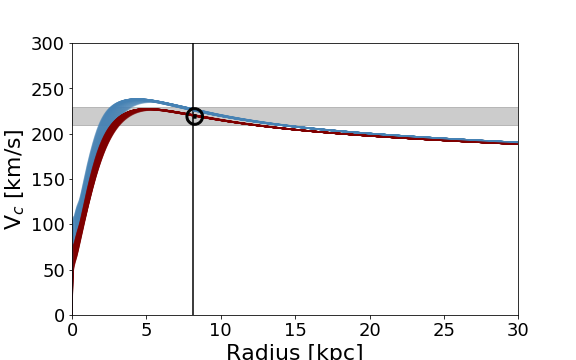
\includegraphics[width=\columnwidth]{v_circ_nlm919.png}}
\caption{\todo{Probably include static potential as well, and show the different components of the potentials }}
\label{fig:vcirc}
\end{figure}



\subsection{Stream modeling}
\label{sec:modeling}
For all simulations we assume a 6D phase space position of Pal 5 as: RA = 229.018 deg, Dec = - 0.24 deg, distance = 22.9 kpc, $v_r$ = -58.7 , pm$_{RA,cosdec}= -2.296$ mas and pm$_{Dec} = -2.257$ mas. We first transform Pal 5's 6D phase space position into a Galactocentric frame by assuming $v_{lsr} = (11.1, 24.0, 7.25) \kms$, 
$v_{circ} = 220  \kms$ and a distance from the Sun to the Galactic centre of 8.1 kpc. 

We integrate the cluster backwards in time for 4 Gyr in steps of 0.5 Myr. Subsequently, we simulate the forward evolution of Pal 5 using the ``particle-spray" stream generating method developed by \citet{Fardal:2015}, such that the cluster ends at its present day position. We release two particles through each of the two Lagrange points every 10 Myr. We repeatedly at this in first the NFW potential setting $q_z = 0.94$ (\citealt{Bovy:2016}) and subsequently in a flattened NFW potential ($q_z = 0.5$ to induce a chaotic orbit). 

Additionally, we simulate the evolution of Pal 5's stream in the barred potential, where we vary the pattern speed from and the bar mass, while updating the physical scaling of the bar (see Section \ref{sec:potential} and Figure \ref{fig:vcirc}). 


\section{Density model}
\label{sec:density}
To compare our data and various Pal 5 simulated streams, we construct density model consisting of a multicomponent Gaussian mixture model. In particular, we are interested in fitting the width and density of our data and various simulations.  

We first transform our simulated Pal 5 data points to the tangent sky plane using a Zeanit (Lambert azimuthal) equal-area projection, such that we can define a Gaussian. We call these coordinates, $X$, $Y$.

We then fit a 3rd order polynomial to the leading and trailing arm separately, in this projected space. 

We place K nodes, k, equally in distance along the polynomial fits to the leading and trailing arm. 

At each node, k, along the polynomial we find the tangent/parallel unit vector,  $\hat{u}$, and the perpendicular normal unit vector, $\hat{v}$, to the stream. 

At each node, k, we define the co-variance matrix, $\tilde{C_k}$:

\begin{equation}
\tilde{C_k} = 
\begin{pmatrix}
    h^2 & 0  \\
    0 & S_k^2  \\
\end{pmatrix}
\end{equation}
where $h$ is bandwidth of the Gaussian components along the polynomial fit and $S_k$ is the  width of the Gaussians in the perpendicular (normal) direction of the stream at any node, k. 

We transform it from the space spanned by the $\hat{u}$,  $\hat{v}$ vectors to $X$, $Y$:
\begin{equation}
C_k = \rm{R} \tilde{C_k} \rm{R}^T
\end{equation}
where
\begin{equation}
\rm{R} = 
\begin{pmatrix}
    \rm{cos} \theta & - \rm{cos} \theta  \\
    \rm{cos} \theta & \rm{cos} \theta \\
\end{pmatrix}
\end{equation}
and  $\theta$ is the angle between the tangent sky plane and the unit vector, $\hat{u}$.

To compute our density model along the leading at trailing stream, for the K nodes, k, we define ln density  and sum over the K nodes:
\begin{equation}
\rm{ln} \sum ( \alpha_k \mathcal{N}\left(\mu_k, C_k\right))
\end{equation}
where $\mu_k$ denotes the location of each node, k, along the leading and trailing polynomial fits, respectively, $C_k$ is the covariance matrix, and $\alpha_k$ is the amplitude of the Gaussian (representing density at specific node, k). 

We then fit for the perpendicular width, $S_k$, to the stream (polynomial fits) and the amplitude of the Gaussians, $\alpha_k$, which represent the density along the stream. 

%Explain background model for data.

We compute the width and density of both or simulated Pal 5 streams and the DECaLS data fitting the above Gaussian mixture model. 


\section{Results}
\label{sec:results}
In this Section, we show the results of modeling Pal 5 in a static potentail with varying halo flattening and in a barred potentials with various pattern speeds and compare the simulations to our data using the density model described in Section \ref{sec:density}.

\subsection{Static Potentials}
The left panel of Figure \ref{fig:static} shows the Pal 5 on a regular orbit in a static potential with a flattening of $q_z = 0.94$ (\citealt{bovy:2017}). The leading and trailing arm of Pal 5 are symmetric, as expected (\citealt{dehnen:2004}, \citealt{Pearson:2015}). In the right panel, we show a stream evolved in a flattened static potential ($q_z = 0.5$), in order to induce a chaotic orbit. For both scenarios the leading and trailing arm look symmetric, although the arms are ``fanned" out in the chaotic case (\citealt{Pearson:2015}, \citealt{Price-Whelan:2016}). 

\begin{figure}
\centerline{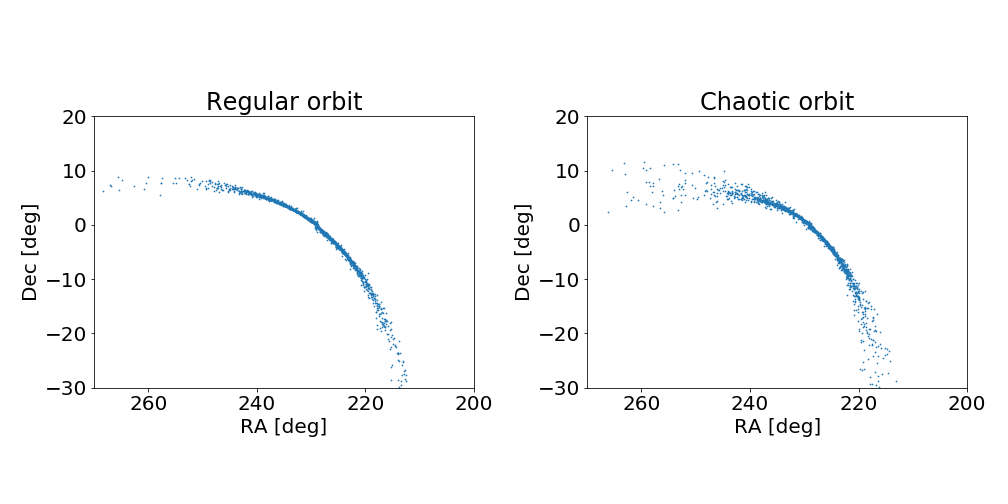
\includegraphics[width=\columnwidth]{static.png}}
\caption{\todo{Placeholder, but maybe only show these two sims. in one fig as Ana suggested. Have panels with our width and density as estimated from the density model. Maybe also show data density model in those panels?}}
\label{fig:static}
\end{figure}

\subsection{Barred Potentials}
In Figure \ref{fig:bar} we show four different simulated Pal 5 streams that all yield densities and widths comparable to the data. These streams were evolved in a barred potential with pattern speeds of $\Omega_b = (...) \kms$ kpc$^{-1}$. We selected these four examples through visual inspection of the density and width of the data and the simulated streams. 


\section{Discussion}
\label{sec:discussion}

\subsection{Other perturbers}
As Pal 5 is moving prograde with respect to the disk it will be subject to interactions with both the bar (\citealt{Hattori:2016}, \citealt{price:2016b}) and molecular clouds (\citealt{amorisco:2016}). Additionally, dark matter substructure could also be interacting with the stream (although probing inner potential: \citealt{Garrison-Kimmel:2017}). 

\begin{itemize}
\item{Molecular clouds}
\item{Spiral arms}
\item{Dark matter subhalos}
\end{itemize}


\acknowledgements{
It is a pleasure to thank


This work has made use of data from the European Space Agency (ESA) mission {\it
Gaia} (\url{https://www.cosmos.esa.int/gaia}), processed by the {\it Gaia} Data
Processing and Analysis Consortium (DPAC,
\url{https://www.cosmos.esa.int/web/gaia/dpac/consortium}). Funding for the DPAC
has been provided by national institutions, in particular the institutions
participating in the {\it Gaia} Multilateral Agreement.  This research was
started at the NYC Gaia DR2 Workshop at the Center for Computational
Astrophysics of the Flatiron Institute in 2018 April.

AB acknowledges generous support from the Institute for Theory and Computation
at Harvard University.
% All code used in this work and all results are available at
% \url{https://github.com/adrn/GD1-DR2}.
}

\software{
    \package{Astropy} \citep{astropy, astropy:2018},
    \package{dustmaps}\footnote{\url{https://github.com/gregreen/dustmaps}},
    \package{gala} \citep{gala},
    \package{IPython} \citep{ipython},
    \package{matplotlib} \citep{mpl},
    \package{numpy} \citep{numpy},
    \package{scipy} \citep{scipy}
}

\bibliographystyle{aasjournal}
\bibliography{pal5fan}

\end{document}
